
\chapter{Time Domain: \polytempic}
\label{ch:polytempic}
In \autoref{ch:introduction} (see figure~\ref{fig:metastasis}) we saw how
Xenakix was using ruled surfaces to create swarms of notes that move
together, creating stochastic sonorities. The goal of \polytempic is
to enable composition with swarms of tempo modulations that move in
correlated, cohesive patterns. Music with two or more simultaneous
tempos (polytempic music) is itself not a new concept, and many
examples of polytemic music exist\cite{Greschak2003}. Slightly less
comon is polytempic music where continuous tempo accelerations or
deccelerations are defined relative to each other.  This style of music
is well suited to tape music, because tape machines can play
recordings back at variable rates. However, it is difficult to control
the exact point (or phase) when de-synchronized tape becomes
re-aligned. Performative music with simultaneous tempi that accelerate
and decelearate realtive to each other is unusual, but does exist. In
a 1971 interview composer Steve Reich described how he made the
transition to performative polytempic music after working on his tape
music composition, \textit{Come Out}:
\begin{quotation}
  ``1966 was a very depressing year. I began to feel like a mad
  scientist trapped in a lab: I had discovered the phasing process
  of Come Out and didn't want to turn my back on it, yet I didn't know
  how to do it live, and I was aching to do some instrumental
  music. The way out of the impasse came by just running a tape loop
  of a piano figure and playing the piano against it to see if in fact
  I could do it. I found that I could, not with the perfection of the
  tape recorder, but the imperfections seemed to me to be interesting
  and I sensed that they might be interesting to listen to.''\cite{Nyman2015}
\end{quotation}
Reich's experience illustrates what other composers and performers
have also encountered: It is quite difficult to perform polytempic
music accurately. In \textit{Piano Phase} Reich has two performers
playing the same 12 tone series on the piano. After a set number of
repetitions through the pattern, one performer begins to play slightly
faster until she is exactly one note ahead of the other performer, at
which point both performers play at the same rate for a time. This
process is repeated and iterated on, creating a live \emph{phasing}
effect without the pitch shifting that would occur when phasing analog
tape. If we compare a live performance\cite{Huisman1989} with a
programatic rendering\cite{Chen2014} of \textit{Piano Phase}, we can
hear how the programatic rendering is able to accelearate more
smoothly. The programatic example spends longer on the transitions
where the two parts are out of phase.

\section{Objective}
\label{sec:polytempic-objective}
Steve Reich composed \textit{Piano Phase} for two performers. In his
experimentation, he found that if the music is reasonably simple, two
performers can make synchronized tempo adjustments relative to each
other well enough to yield compelling results. To create stochastic
tempo transitions, our requirements are probably too demainding for
unassisted performers. Our goal is to compose and audition music
where:
\begin{enumerate}
  \item Swarms of an arbitrary number of simultaneous tempi
    coexist. 
  \item Each individual player within the swarm can continously
    accelerate or decelerate individually, but also as a member of a
    cohesive whole. 
  \item Each musical line can converge and diverge at explicit
    points. At each point of convergence the phase of the meter within
    the tempo can be set.
\end{enumerate}
We start by defining a single tempo transition. Consider the following
example (shown in figure~\ref{fig:basic-tempo-change}):
\begin{itemize}
\item Assume we have 2 snare drum players. Both begin playing the same
  beat at 90 BPM in common time.
\item One performer gradually accelerates relative to the other. We want
  to define a continous tempo curve such that one drummer accelerates
  to 120 BPM.
\item So far, we can easily accomplish this with a simple linear tempo
  acceleration. However, we want the tempo transition to complete
  exactly when \emph{both} drummers are on a down-beat, so the the
  combined effect is a 3 over 4 rhythmic pattern. \textbf{Linear
    acceleration results in the transition completing at an arbitrary
    phase.}
\item We want the accelerating drummer to reach the new tempo after
  exactly 20 beats.
\item We also want the acceleration to complete in exactly 16 beats of
  the original tempo, so the drumer playing a constant tempo, and the
  the accelerating drummer are playing together.
\end{itemize}
\begin{figure*}[h]
  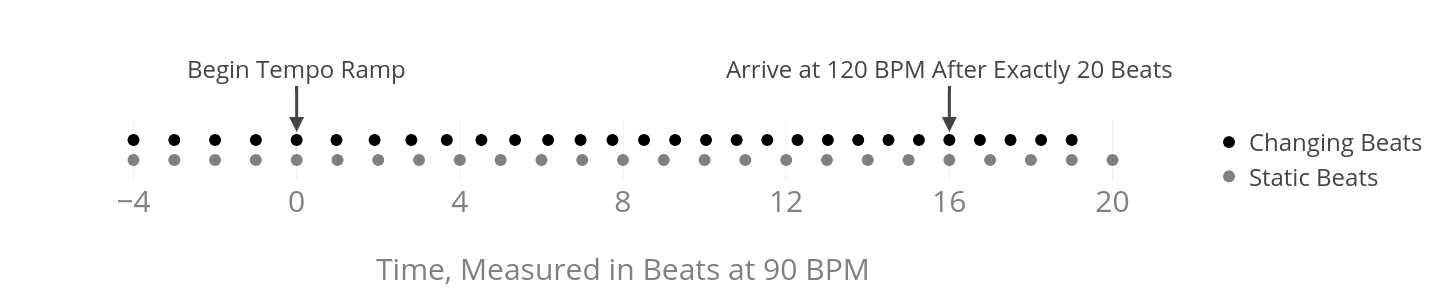
\includegraphics[width=\linewidth]{basic-tempo-transition.png}
  \caption[Tempo Transition]{Tempo Transition from 90~BPM
    to 120~BPM}
  \label{fig:basic-tempo-change}
\end{figure*}

\section{Solution}
\label{sec:polytempic-solution}
We are interested in both the number of beats elapsed in the static
tempo \emph{and} in the changing tempo, and the absolute tempo. Let us
think of the number of beats elapsed as our \emph{position}, and the
tempo as our \emph{rate}, we see how this resembles a physics
problem. If we have a function that describes our tempo (or rate), we
can integrate that function, and the result will tell us our number of
beats elapsed (or position). Given the above considerations, we define
our tempo curve in terms of 5 constants:
\hfill\break
\begin{fullwidth}
\begin{itemize}
  \item Time $t_0=0$, when the tempo transition begins
  \item A known time, $t_1$, when the tempo transition ends
  \item A known starting tempo, $\dot{x}_0$
  \item A known finishing tempo, $\dot{x}_1$
  \item The number of beats elapsed in the changing tempo between
    $t_0$ and $t_1$, $x_1$
\end{itemize}
\end{fullwidth}
\hfill\break
The tension of the tempo curve determines how many beats elapse during
the transition period. The curve is well-defined for some starting
acceleration $a_0$ and finishing acceleration $a_1$, so we define the
curve in terms of linear acceleration. Using Newtonian notation we can
describe our tempo acceleration as:
\begin{equation}
	\label{accel}
    \ddot{x}_1 = a_0 + a_1t_1
\end{equation}
Integrating linear acceleration (\ref{accel}) yields a quadratic
velocity curve (\ref{bpm}). The velocity curve describes the tempo (in beats per
minute)\marginnote{We must specify the same time units for input
  variables like $t_1$ and $\dot{x_1}$. I prefer \textit{minutes} for
  $t_1$ and \textit{beats per minute} for $\dot{x_1}$ over
  \textit{seconds} and \textit{beats per second}} with respect to
time.
\begin{equation}
	\label{bpm}
    \dot{x}_1 = \dot{x}_0 + a_0t_1 + \frac{a_1t_1^2}{2}
\end{equation}
Integrating velocity (\ref{bpm}) gives us a function describing
position (the number of beats elapsed with respect to time).
\begin{equation}
	\label{beats-elapsed}
	x_1 = x_0 + \dot{x}_0t_1 + \frac{a_0t_1^2}{2} + \frac{a_1t_1^3}{6}
\end{equation}
With equations (\ref{bpm}) and (\ref{beats-elapsed}), we can solve for our 
two unknowns, $a_0$ and $a_1$. First we solve both equations for $a_1$:
\begin{displaymath}
    \label{a1-solution}
    a_1=
    \frac{-2}{t_1^2}(\dot{x}_0-\dot{x}_1 + a_0t_1)=
    \frac{-6}{t_1^3}(\dot{x}_0-x_1 + \frac{a_0t_1^2}{2})
\end{displaymath}
Assuming $t_1 \neq 0$, we solve this system of equations for $a_0$:
\begin{equation}
	\label{a0-result}
	a_0=\frac{6x_1-2t_1(\dot{x}_1+2\dot{x}_0)}{t_1^2}
\end{equation}
Evaluating (\ref{a0-result}) with our constants gives us our starting
acceleration. Once we have $a_0$ we can solve (\ref{bpm}) for $a_1$, and 
evaluate (\ref{bpm}) with $a_1$ and $a_0$ to describe our changing tempo 
with respect to time.

\section{Stochastic Transitions}
\label{sec:polytempic-implementation}
Equiped with out equations from the previous section, it is quite
simple to create swarms of parallel tempos that are correlated and
complex. In figure~\ref{fig:polytempic-transition} we build on the
previous example. Here, each additional tempo curve is calculated the
same way, except $x_1$ (number of beats in our accelerating tempo
during the transition) is incremented for each additional tempo line. 
\begin{figure*}[h!]
  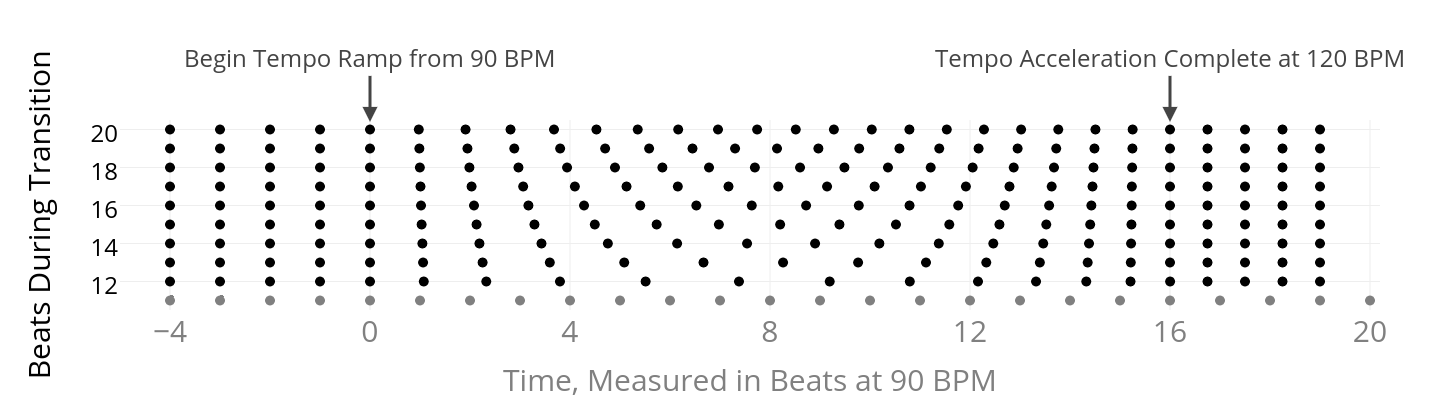
\includegraphics[width=\linewidth]{stochastic-tempi.png}
  \caption{Stochastic Tempo Transition from 90~BPM to 120~BPM. Black
    dots are beats in our changing tempi. Grey dots are static
    beats at the original tempo. $12 \leq x_1 \leq 20$}
  \label{fig:polytempic-transition}
\end{figure*}\hfill\break
This pattern clearly exhibits controlled chance, and that Xenakis
would describe as \emph{stochastic}. On the very first beat at $t=0$,
all parallel parts are aligned. Beats 2 and 3 can be heard as discrete
rythmic events, but become increasingly indistinct. The end of beat 4
then overlaps with the beginning of beat 5 as individual beats slide
into psuedo random noise. By beat 13 of the static tempo, the chaos of
the many accelerating tempi begin to settle back into order before
returning to complete syncronicity at $t=16$.

\section{Implementation}
\label{sec:polytempic-implementation}

Bryn Bliska Tide

\section{Polytempic Music and Polymetric Music}
\label{sec:polytempic-vs-polymetric}
It is easy to confuse poly tempic music with polymetric music.  Pieces
where multiple meter
Other notable composers
of the time include John Cage, who wrote wrote what he called, Chance
Music, and Stockhausen, Boulez and Berio who wrote aleatoric music.


Eliot Carter: Polymetric Modulation. 
Steve Reich: Piano Phase
Paper: realtime representation of 
Paper: Stochos: Software for Real-Time Synthesis of Stochastic Music

John Cage: Chance Music
Karlheinz Stockhausen, Pierre Boulez, Luciano Berio: Aleatoric music

\section{Contribution}
\label{sec:polytempic-contribution}

and finishes the tempo transition slightly different tempos.

To audition stochastic tempo transitions, we can create software tools
that promt musicians with visual cues or aural cues, 
More flexible Digital Audio Workstations (DAWs) like Reaper and
Digital Performer include workarounds for auditioning simultaneous
tempo. 

For example we 

Xenakis was among a group of
20th century composers who were searching for ways to push the
boundaries of established music composition.


%%% Local Variables:
%%% mode: latex
%%% TeX-master: "CharlesHolbrow_MAS_Thesis"
%%% End:
